\chapter{State-of-the-Art}\label{chap:state-art}
In the demand for an effective, high-quality approach to the analysis of isolates from infected animals, molecular studies help to investigate characteristics of the sample. Genome analysis has become an integral part of animal disease surveillance, especially since the advent of high-throughput sequencing technologies in the last 15 years. Next-generation techniques, applications and drawbacks are described below, software tools to use handle NGS data, state of the art in poxvirus and avian influenza virus analysis, and lastly pipelines for genomic analysis are discussed.

\section{High-throughput Technologies in Genomics and Virology}
When comparing \ac{DNA} sequencing technologies, there are differences in speed, throughput and volume of sequences. The term ``next-generation'' in \ac{NGS} is used to describe newer technologies in the field and implies a next step in the evolution of sequencing technologies. As sequencing machine technologies evolve rapidly, there are gradations such as ``second-generation'' and ``third-generation''. Following the original 1977 Sanger sequencing method using radioactivity and gels, second-generation sequencers are advancements of Sanger sequencing that applies sequencing by synthesis~\cite{mardis2008next}. In second-generation methods, reactions run in parallel and drastically reduce overall costs compared to Sanger sequencing. They produce short sequence read length and are able to detect reads without using electrophoresis. Reads are equal to single fragments of \ac{DNA} or \ac{RNA}.
Third-generation sequencing technologies typically generate longer primary reads of \ac{DNA} or \ac{RNA} molecules while maintaining the massive parallelism of the technology and taking advantage of this benefit~\cite{slatko2018overview}. The nowadays most commonly used next-generation technologies for sequencing and their applications are described below.

\subsection{NGS Platforms and Applications}
By far the biggest player in the field of \ac{DNA} sequencing is the Illumina platform, first developed by Solexa and Lync Therapeutics~\cite{illumina2015introduction}. Illumina sequencing is based on bridge amplification, which creates clusters of copies of each \ac{DNA} fragment. This technique involves repeated synthesis reactions with proprietary modified nucleotides containing a different fluorescent label for each of the four bases A, T, C and G. The reactions are performed over 300 or more rounds, and fluorescent detection allows for faster detection through direct imaging. An Illumina sequencer outputs data in the form of sequence reads, which are short \ac{DNA} fragments ranging from 50 to 600 base pairs in length depending on the specific instrument and protocol used~\cite{illumina2015introduction, slatko2018overview, mardis2008next}. Error rates of Illumina MiSeq and HiSeq sequencers range from 0.1\% to 10\% depending on the experiment and platform used~\cite{illumina2015introduction}. The output data from an Illumina sequencer typically is in the form of raw sequence files in FASTQ format, which contain the base calls and corresponding quality scores for each read. These reads can be used for downstream analyses such as viral genome assembly and variant calling.

\ac{ONT} is a third-generation paradigm shifting sequencing technology. It measures changes in ionic current across membranes as single-stranded \ac{DNA} nucleotides pass through a nanopore~\cite{jain2016oxford}. Nanopore-based \ac{DNA} sequencing technologies are purchasable as a portable, small MinION (by \ac{ONT}) device, allowing experts to use it for applications where space requirements or portability are important~\cite{greninger2015rapid, jain2016oxford}. The cyclic mode of sequencing used in second-generation approaches is replaced by sequencing in real-time with read lengths of up to 10,000 basepairs~\cite{jain2016oxford}. Despite its advantages, the main caveat of \ac{ONT} is its relatively high error rates of 10\% to 15\% compared to other \ac{HTS} methods~\cite{fu2019comparative, laver2015assessing}. This makes \ac{ONT} less suitable for single-nucleotide variant analysis that is required in some diagnostic applications~\cite{bowden2019sequencing, stefan2022comparison}. \\
Other frequently used second-generation platforms are Roche/454 sequencing, IonTorrent (Thermo Fisher) technology and SOLiD (Sequencing by Oligonucleotide Ligation and Detection). Third-generation platforms include \ac{SMRT} by PacBio and nanopore sequencing~\cite{rhoads2015pacbio}. 

\begin{figure}[ht!]
	\centering
	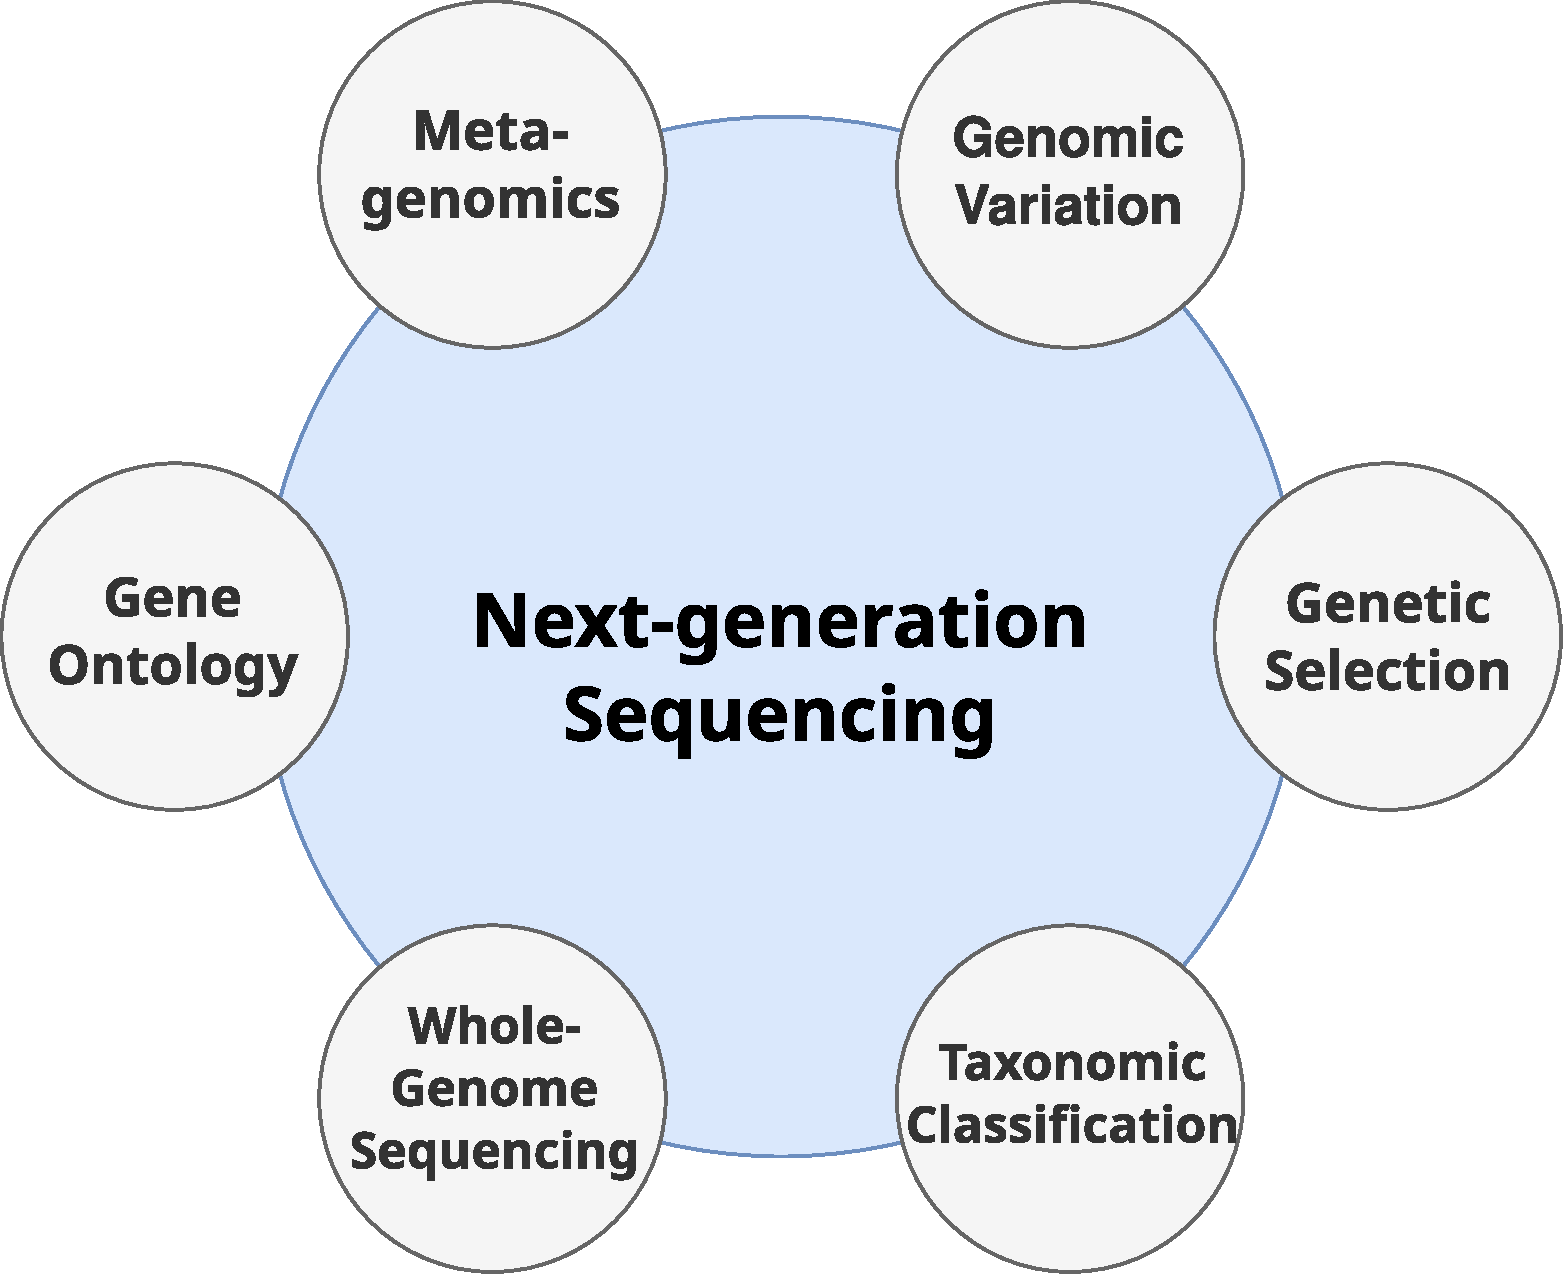
\includegraphics[width=0.7\textwidth]{media/2-ngs.pdf}
	\caption{Next-generation sequencing technology applications in virology.}
	\label{fig:2-ngs}
\end{figure} 

As \ac{NGS} platforms are widely used in biomedical and clinical contexts, some of the most important applications in diagnostic virology are depicted in~\figref{fig:2-ngs}. In virology, metagenomics can be used to identify viruses in complex clinical or environmental samples~\cite{chiu2019clinical}. It allows for the detection of known and novel viruses without prior knowledge of the infectious agent. Metagenomics involves the sequencing of all genetic material in a sample, including viral genomes, to identify the presence of viruses. Once a virus is identified, genomic variation refers to differences in the \ac{DNA} sequence of a virus between different strains or isolates. These variants can be used for tracking the spread of an outbreak, identification of sources of an infection, or information about virus virulence~\cite{capobianchi2013next}. Variant detection is only possible with the sequenced genome, as it provides insight to the genome on a nearly every-base level and allows to reliably interpret and identify the many different possible variants~\cite{koboldt2013next}. \\ 
Genetic selection describes the process by which certain viral strains become more prevalent in a population over time due to selective pressures. In genomics with viral material, genetic selection is used to track the evolution of a virus in the course of time and determine which strains are most likely to cause outbreaks or epidemics. This is of special interest in the backtracing of infected animals to know where the virus came from. Using gene ontology, functions and interactions of genes are described. This is crucial to identify the genes responsible for specific viral functions and to understand how these functions contribute to viral pathogenesis and transmission. \\
Based on their genetic and structural characteristics, viruses are classified to existing systems, called taxonomic classification. This clustering analysis can be used for the type identification of a virus causing infections and determination of its potential for transmission or pathogenicity~\cite{dutilh2021perspective}.\\
Whole-genome \textit{de novo} assembly is the reconstruction of an entire viral genome without prior knowledge of its genetic sequence, being a costly and time-intense method with potentially high error rates. Similar to metagenomics, whole-genome sequencing and assembly can be used to identify novel viruses, to study mutations in viral genomes and to track the evolution of a virus over time~\cite{slatko2018overview}. In contrast, transcriptomic sequencing is used for viral identification of viruses that are actively expressed in their host, and is performed at a fraction of the cost needed for \ac{WGS}.

For \ac{NGS} methods to be a viable tool in diagnosis and analysis of viral animal diseases, the methods must be efficient and reliable. Almost all downstream analyses depend on the data obtained by sequencing, hence it is imperative to choose the most appropriate method for each application. \\
The reconstruction from \ac{HTS}-generated reads to assemble the full-length genome can be made using different approaches, depending on the preparation of the \ac{NGS} data and the objectives. During sequencing, \ac{PCR} amplification on the whole genome is a widely used technique to amplify specific regions of nucleic acids by producing many copies of the targetted sequence. \ac{PCR} is used to sequence for example specific genes in a viral metagenomic sample. Another approach, developed by the ARTIC network is based on amplicons, i.e. fragments of the genetic sequence that cover the whole genome and are then sequenced on an Illumina platform. Amplicons are generated by tiled primers that start a \ac{PCR} to generate the amplicons. For each amplicon, two primers for each end of the region of interest are needed, hence the expression tiled or tiling primers. The distance between the primers determines the size of the produced amplicon~\cite{mamanova2010target}.

\subsection{Data Analysis Issues}
Since the surveillance of viral animal diseases with \ac{NGS} is advancing rapidly, it is important that regions and health organisations that experience high damage of viral outbreaks but do not have their own facilities and know-how have access to the needed tools and knowledge. Costs for \ac{NGS} sequencers are high and the access to appropriate laboratories is not given everywhere. Networks like \ac{VETLAB} and standardisation of techniques, for example freely available and published by the \ac{WOAH}, can enable professionals worldwide independent of their equipment on site. In the scope of the \ac{ZODIAC} project, this aspect is addressed by providing protocols for each step from taking samples of potentially infected animals to the detailed analysis and derived actions~\cite{zodiac2021}.

\ac{NGS} methods themselves have downsides that need to be considered when applying these techniques. Generally, chimerical sequences are formed during sequencing, which may be interpreted as false positives for novel organisms if the data are not cleaned. Chimeric products are artefacts originating from joining sequences and are represented by point mutations, insertions and deletions. Chimera formation also occurs during \ac{PCR} amplification~\cite{zylstra1998pcr}.\\
During bioinformatics analysis steps using algorithms with computationally expensive steps, the choice of the algorithm as well as its configuration settings have huge impact on the final results. This includes algorithms in steps such as quality filtering, clustering and sequence classification~\cite{kopylova2016open}. The cleaning step or filtering phase eliminates low-quality reads from the dataset, whereas the error correction process distinguishes true variants from those caused by experimental noise. This is based on the concept that errors occur randomly with low frequency, while true mutations tend to be clustered, and their frequency can be measured~\cite{zagordi2010error}. Longer reads preclude this problem because contigs must not be assembled in the first place, avoiding clustering and filtering errors. This is why the shift in third-generation and later sequencing platforms is towards longer reads again. Due to the relatively high error rates of \ac{HTS} technologies that base on the sequencing process itself, \ac{PCR} amplification of the viral material and reverse transcription of viral \ac{RNA} to \ac{cDNA}, it is crucial to include quality checks and filtering steps when using the \ac{HTS} data~\cite{beerenwinkel2012challenges}. \\
Each application of software used with \ac{NGS} data requires expertise in resolving limitations and drawbacks of specific methods. This in turn requires skills and experience in the field and the careful interpretation of results. Nevertheless, \ac{NGS} technologies provide a large pool of methods, although also available algorithms for genome assembly and amplicon analysis have drawbacks and limitations~\cite{finotello2012comparative}.

\section{Tools for Genomic Analysis with NGS Data}
A variety of suites and software packages is available to process NGS-generated data. Depending on the user's research and analysis interest, tools are used independently and/or subsequently. A tool represents a modular program to use with data input from the user. Different suites for bioinformatical analyses offer different interfaces to execute a tool, either on the commandline to work on a server, or via a web-interface. The software of a tool can be complex algorithms and expensive calculations, or simple and fast formatting programs. \\
Pursuing the goal to construct the full-length genome, short NGS-sequenced raw reads in FASTQ format, which is the text-based standard format to store nucleotide sequences with numeric quality scores for each nucleotide, serve as the primary input for any analysis steps. For the central steps of the bioinformatics pipelines described in \secref{sec:2-pox-pipelines}, \secref{sec:2-aiv-pipelines}, \secref{sec:2-general-pipelines} and importantly the newly designed pipelines in \secref{sec:pox-wf}, \secref{sec:aiv-wf} and \secref{sec:fmdv-wf}, tools and software suites that can work with NGS-generated data from different techniques are discussed in the following. 

\subsubsection*{Tools for Preprocessing}
Working with raw NGS reads requires quality control before executing any further steps. Preprocessing with quality control helps the user to understand the sequencing data and to check its overall quality so sequencing errors, PCR artefacts and contaminations can be detected. Usually, a quality filtering to keep only reads above a certain length and quality threshold is conducted in the preprocessing, as well as when working with ampliconic data, trimming typical sequencing artefacts. The remnants of adapters, artifically introduced during sequencing, need to be removed as they are not part of the transcriptome. Common tools for this purpose are \texttt{FastQC}, \texttt{Trimmomatic}, \texttt{Cutadapt} or \texttt{fastp}~\cite{andrews2010fastqc, bolger2014trimmomatic, martin2011cutadapt, chen2018fastp}. Being developed specifically for adapter-trimming of Illumina and SOLiD data, \texttt{Cutadapt} is a commandline tool written in Python that at the time of publishing was the only tool to support colour-space data. It also provides some read-filtering options~\cite{martin2011cutadapt}. \texttt{Trimmomatic} was developed to solve similar tasks but with higher performance and correct handling of paired-end data. It works with Illumina sequenced data and the user can upload the adapter sequences for adapter trimming if they deviate from standard protocols. It performs quality pruning with a sliding-window cutting algorithm~\cite{bolger2014trimmomatic}. \texttt{FastQC} is a Java-based tool for quality control and provides per-base and per-read quality profiling options~\cite{andrews2010fastqc}. The newest tool for preprocessing \texttt{fastp} provides an all-in-one solution for quality control of FASTQ data, which includes all of the options the formerly mentioned tools provide. Additionally, \texttt{fastp} outperforms them in terms of speed by being 2 to 5 times faster~\cite{chen2018fastp}. From the point of view of the user who wants to perform all the steps of quality control, filtering and trimming, none of the tools except \texttt{fastp} offers all the functions, which slows down the preprocessing because several tools have to be started. Additional features such as unique molecular identifier preprocessing and per-read polyG tail trimming are integrated into \texttt{fastp}~\cite{chen2018fastp}. Its multithreading implementation in C/C++ makes it much faster than the previously mentioned tools. Reporting of the quality results to compare statistics of the reads before and after the preprocessing run is possible with all tools in combination with \texttt{MultiQC}~\cite{ewels2016multiqc}.

\subsubsection*{Tools for Alignment}
In order to obtain the full-length sample sequence and to identify \acp{SNP} in an isolate, short sequenced reads need to be aligned to a reference genome. Assembly of short reads can also be done as \textit{de novo} assembly without a reference, however this approach requires greater computational capacities and greater sequencing depth to ensure a sufficient overlap of the reads for an accurate assembly~\cite{ekblom2014field}. \\
The choice of alignment method depends on the amount, length and origin of read data. For reference-based alignment approaches, typically \texttt{minimap2} is used with \ac{ONT}, PacBio or Illumina-sequenced data. \texttt{minimap2} is a pairwise aligner for short reads of at least 100 basepairs in length~\cite{li2018minimap2}. It states to be faster and more accurate than other domain-specific alignment tools~\cite{li2018minimap2}. \\
Other frequently used tools are \texttt{BWA-MEM} for Illumina data and \texttt{Bowtie2} for \ac{ONT} data. Like most other full-genome aligners, \texttt{BWA-MEM} follows the seed-chain-align pattern~\cite{li2013aligning}. Using a Burrows-Wheeler Transform, both \texttt{BWA-MEM} and \texttt{Bowtie2} are shown to be faster aligners than others with reads of 100 basepairs in length~\cite{borozan2013evaluation}. \\
For \textit{de novo} assembly with Illumina, PacBio or IonTorrent data, \texttt{SPAdes} is used. It is based on a De Bruijn graph algorithm by building k-mers~\cite{bankevich2012spades}. For \ac{ONT} or PacBio data to align long error-prone reads, \texttt{Flye} is a modern \textit{de novo} assembler, shown to be highly performant with relatively low error rates~\cite{kolmogorov2019assembly, dida2021empirical}. Its underlying algorithm is A-Bruijn assembly graph construction that attempts to generate arbitrary paths with overlaps, unlike other De Bruijn-based assemblers which attempt to generate long accurate contigs~\cite{kolmogorov2019assembly}. 

\subsubsection*{Consensus Sequence Construction}
Representing the alignment results in the form of a full-length genome, based on the calculated order of the most frequent residues for each position the consensus sequence is constructed. With aligned Illumina reads, the \texttt{iVar} suite provides tools to generate the consensus sequence. Its features also include primer and quality trimming (\texttt{iVar trim}) and intrahost variant detection (\texttt{iVar variants})~\cite{grubaugh2019amplicon}. On the \texttt{Geneious} platform, similar analyses can be executed in order to produce a consensus sequence from raw reads\cite{kearse2012geneious}. \texttt{bcftools} as a tool suite also offers a package for consensus sequence construction from \ac{VCF} files~\cite{li2009sequence}.\\
For \ac{ONT} generated data, the \texttt{medaka} tools suite provides a module to generate the consensus sequence. 

\subsubsection*{Phylogenetic Tree Construction}
Having multiple virus strain samples and wanting to express their relations, evolutionary or phylogenetic trees are a common method to use with nucleotide sequences. Most common tools are \texttt{FastTree} and \texttt{IQ-Tree}, both based on infering relations using the maximum-likelihood criterion~\cite{price2009fasttree, minh2020iq}. Other, more inefficient algorithms rely on creating a distance matrix to compute the minimum distances. Both \texttt{FastTree} and \texttt{IQ-Tree} require a multiple sequence alignment as input data, which can be obtained by multiple sequence aligners like \texttt{MAFFT} or \texttt{ClustalW}~\cite{katoh2013mafft, thompson2003multiple}. Generated phylogenetic trees can be visualised to infer topologies and study relationships of taxon-groups, while only the \texttt{IQ-Tree} tool provides an in-built visualisation in \textit{iqtree} format. With the phylogenetic tree in Newick format (\textit{nhx}) and the \texttt{PhyloCanvas} tree viewer, trees can be exported, extended and visualised with other tools~\cite{abudahab2021phylocanvas}.

\subsubsection*{Classification of Sequences}
Many applications of genomic analysis require the placement of the inferred sequence compared to other, similar sequences. There are many databases available for different categories of sequences, offering database searches to find the closest sequence compared to the given sequence. \ac{BLAST} is a popular program to search databases, while there are different heuristics and variations depending on the specific database and search string characterisations~\cite{altschul1990basic}. For nucleotide sequences and databases, the \ac{NCBI} provides a web-based \texttt{\ac{BLAST}} search~\cite{johnson2008ncbi, altschul1997gapped}. The underlying algorithm is a similarity measure that ``permits a tradeoff between speed and sensitivity'' by setting a threshold parameter~\cite{altschul1997gapped}. \\
Having BLAST classifying full-length genomes, short sequencing reads can be used for a database search, too. Specifically developed for and tested with influenza reads, \texttt{VAPOR} is a software tool that infers a scoring based on a De Bruijn graph construction and emits the closest sequences from a database~\cite{southgate2020influenza}. It directly maps reads to a De Bruijn graph without prior assembly and therefore accelerates the classification search as compared to a BLAST search while still achieving similar or better results~\cite{southgate2020influenza}. \texttt{VAPOR} provides options to finetune the classification run, depending on read length, database size, k-mer size and other measures. It also has the option to output a file with the scoring, generated by a scoring function that favours sequences with a high coverage of the reference and with a high weight in the De Bruijn graph~\cite{southgate2020influenza}.

\section{Pipelines for Genomic Analysis with Viral NGS Data}\label{sec:2-general-pipelines}
In the following, pipelines are presented that can be used with unspecified or unknown virus data. They cover some general parts of the later mentioned pipelines but focus mainly on virus discovery, assembly and consensus sequence generation. \\
ViReflow is a pipeline for viral consensus sequence generation and provides a mapping-based approach to variant calling and many optional downstream analyses such as \textit{de novo} assembly and lineage assignment~\cite{moshiri2022vireflow}. The pipeline is based on the Reflow suite, and all computations run in an \ac{AWS} container in a cloud. Reflow emphasises versioning, testing and workflow sharing and does not provide a user-friendly web interface. Instead, it is accessible via a command-line interface. The user chooses from a tool pool of read trimmers, mappers, variant callers and optional downstream analyses. Defaults are \texttt{iVar} for trimming, \texttt{minimap2} for mapping, \texttt{LoFreq} as a variant caller and consensus sequence calling with \texttt{bcftools}. As a result, it may not be as easy to use as Galaxy and its workflows, including workflow development, as this requires programming in Go language. Similar to other pipelines, ViReflow was originally created for the consensus genome construction of \ac{SARS-CoV-2} samples and has been extended for use with all viral genomes~\cite{moshiri2022vireflow}. \\
Another automated pipeline for viral genome assembly, lineage assignment, mutation and intra-host variant detection is V-Pipe, a computational pipeline assessing genetic diversity and introducing a new alignment method \textit{ngshmmalign} specifically for small and highly diverse viral genomes. It includes local and global haplotype reconstruction and a module for detection of flow cell cross-contamination~\cite{posada2021v}. Although V-Pipe is suitable for all viral genomes, it was tested for the identification of the eight influenza segments and successfully identified them from the test sample. V-Pipe is based on Snakemake as a workflow and dependency manager. \\
Other freely available pipelines for the analysis of viral genomes from \ac{NGS} data with several focuses in genomics are VirFind~\cite{ho2014development} and \ac{IRIDA}~\cite{matthews2018integrated}. These pipelines focus on rapid identification of viral materials and do not provide steps for detailed downstream analyses. Automated pipelines for metagenomic \ac{NGS} data are \ac{drVM} and VirMAP~\cite{lin2017drvm, ajami2018maximal}. However, they do not consider the segmented influenza genome and do not provide output data for custom downstream analyses. To our knowledge, there is no freely available pipeline that uses a mapping-based approach that focuses on the viral segments of the \ac{AIV} genome and uses the closest possible reference for each segment. For the various possible downstream analyses, depending on the specific research question, it is critical for a pipeline to provide data outputs and endpoints that enable user-specific assays. This holds not only for avian influenza virus samples, but also for isolates containing other viral material. Galaxy workflows covering the above points for Illumina-sequenced data have been developed in this thesis and are described in \chapref{chap:methods}.

\section{Poxvirus Analysis}\label{sec:2-pox}
Among the family of poxviruses, there are some diseases that circulate in livestock and pose a risk so that they are on the list of notifiable animal diseases. Among others, mpox, sheeppox and goat pox are the diseases of concern. In the following, characteristics of poxviruses and current approaches to analyse \ac{NGS} data of poxviruses are described.

\subsection{Poxviruses}
Throughout human history, poxviruses have played a significant role with variola being the most notorious as it is the causative agent of smallpox. Smallpox has been described in Chinese texts dating back to the 4th Century AD, and evidence of pox-like scars found on Egyptian mummies suggests the disease may have existed as far back as the 2nd millennium BC~\cite{fenner1988history}. The discovery of a vaccine for smallpox made it the first disease to be eradicated by human efforts, so variola was the first human virus to be successfully eliminated~\cite{fenner2000adventures}. Modern vaccinology owes its origins to Edward Jenner's discovery in the late 18th century that zoonotic infections with the ``cowpox virus'' provided immunity to smallpox~\cite{fenner1988history}. Furthermore, vaccinia virus, which is now used for smallpox vaccination, was the first animal virus to be observed using electron microscopy and the first to be utilized as a vector for transporting foreign genes into animals. This is why poxviruses are among the best-studied viruses. \\
The family of poxviruses, \textit{Poxviridae}, is a family of double-stranded \ac{DNA} viruses. Its natural hosts are vertebrates and arthropods and there are currently 83 species within 22 genera in this family. The \textit{Poxviridae} family is divided into two subfamilies, \textit{Entemopoxvirinae} (insect-infecting viruses) and \textit{Chordopoxvirinae} (vertebrate-infecting viruses). \\
Historically, poxviruses were classified based on disease symptoms and the animal species that was infected. Humans, cows, sheep, goats, horses and pigs have been studied to determine not only clinical symptoms but with the aim to classify poxviruses. This genus classification has been confirmed by recent comparative genome analysis~\cite{gubser2004poxvirus}. Symptoms of disease caused by a poxvirus infection are skin lesions that can differ in size. Depending on the type of poxvirus, the papules can vary from small and pearly papules in infections of \ac{LSDV} to larger crusts and spread generalised pustules in infections with the variola virus. Other general symptoms include fever, headache and rash.

\begin{table}[H]
	\centering
	\begin{tabular}{lll}
	\toprule
	\textbf{Genus}      & \textbf{Virus Species}                          & \textbf{Natural Hosts}                      \\ \midrule
	Avipoxvirus         & Canarypox virus                                 & Songbirds 									\\ 
						& Fowlpox virus                                   & Chickens, turkeys                           \\ \midrule
	Capripoxvirus       & Sheeppox virus                                  & Sheep                                       \\
	                    & Lumpy skin disease virus                        & Cattle                                      \\ \midrule
	Centapoxvirus       & Yokapox virus\textsuperscript{1}                & Humans, mosquitoes                          \\ \midrule
	Cervidpoxvirus      & Deerpox virus                                   & Deer                                        \\ \midrule
	Crocodylidpoxvirus  & Crocodilepox virus                              & Crocodiles                                  \\ \midrule
	Leporipoxvirus      & Myxoma virus                                    & Rabbits, hares                              \\ \midrule
	Molluscipoxvirus    & Molluscum contagiosum virus\textsuperscript{1}  & Humans, primates, birds, dogs               \\ \midrule
	Orthopoxvirus       & Variola virus (Smallpox)                        & Humans (eradicated)                         \\ 
						& Mpox virus\textsuperscript{1}                   & Humans, primates                            \\ 
						& Cowpox virus\textsuperscript{1}                 & Humans, cats, cows, elephants               \\ 
						& Vaccinia virus\textsuperscript{1}               & Humans, cattle, buffalos, rabbits           \\ 
						& Camelpox virus                                  & Camels                                      \\ \midrule
	Parapoxvirus        & Pseudocowpox virus\textsuperscript{1}           & Humans, cattle                              \\ 
						& Orf virus\textsuperscript{1}                    & Humans, sheep, goats, etc.                  \\ \midrule
	Suipoxvirus         & Swinepox virus                                  & Pigs                                        \\ \midrule
	Yatapoxvirus        & Yaba monkey tumour virus\textsuperscript{1}     & Humans, rhesus monkeys                      \\ \bottomrule
	\textsuperscript{1} Zoonotic disease &                                &                                             \\
	\end{tabular}
	\caption{Representative viruses from ten Chordopoxvirus genera.}
	\label{tab:2-chordopox}
\end{table}

\tabref{tab:2-chordopox} shows ten representatives of the 18 Chordopoxvirus genera according to the newest \ac{ICTV} Taxonomy Release from 2021, while at least five genera contain zoonotic poxviruses~\cite{tax2021virus}. Orthopoxviruses have the biggest impact on human and animal health, and are remarkable for their broad host spectrum ranging from humans to wild and domestic animals~\cite{fenner2000adventures}.
The Chordopoxvirus subfamily is characterised by its large, linear double-stranded genome. Size varies between 134 to 365 kilobases~\cite{brunetti2003complete, tulman2004genome}. Chordopoxvirus genomes contain 130 to 328 \acp{ORF}, and typically, two identical \acp{ITR} are located at both ends of poxvirus genomes. \\
Vaccination is available for smallpox, and the vaccine is even considered protective against symptoms of all orthopoxvirus infections. It is recommended for laboratory staff that works with mpox, cowpox, vaccinia and variola~\cite{cono2003smallpox}. For animals, there is a smallpox-based vaccine that is used to protect elephants against cowpox~\cite{kurth2008rat}. Sheep and goats are broadly vaccinated with an orf vaccine, which is, similar to smallpox vaccine, a live virus. The effective vaccination against existing poxvirus diseases and further microbiological studies, as well as similarities between poxviruses, motivate the expansion of existing data analysis pipelines that work for a specific poxvirus so that they can also work with other poxviruses.

\subsubsection*{Lumpy Skin Disease Virus}
\ac{LSD} is caused by the lumpy skin disease virus belonging to the \textit{Capripoxvirus} (CaPV) genus within the family of poxviruses, subfamily \textit{Chordopoxvirinae}~\cite{walker2019changes}. The \ac{LSD} virus genome is a double-stranded linear \ac{DNA} molecule of circa 151 kilobasepairs in length. It contains between 147 and 156 open reading frames. Similar to other poxviruses, the \ac{LSDV} genome consists of a central coding region which is bounded by two identical \ac{ITR} regions with a length of circa 2,400 basepairs at both ends of the genome. This is a key characteristic to consider during reconstruction of the genome. With a sequence identity of over 96\% with the other \acs{CaPV} genus members sheeppox and goatpox, the \ac{LSDV} genome is highly similar to the other \acs{CaPV} genomes~\cite{tulman2001genome}. \\
\ac{LSDV} is not known to be transmissible to humans and therefore not a zoonosis. Natural hosts of \ac{LSDV} are cattle and Asian water buffalos. Although \acs{CaPV} is considered to be host specific, sheeppox and goatpox strains can naturally cross-infect in both host species. There have been no cases of natural infection of sheep or goats with \ac{LSDV} reported~\cite{namazi2021lumpy}. The three \acs{CaPV} viruses are the most serious poxvirus diseases of livestock in terms of economic losses in the case of an outbreak. \\
Cattle infected with the \ac{LSDV} typically show symptoms like fever, reduced feed and water uptake and characteristic skin nodules. The number of lesions varies from a few to many, covering the whole body~\cite{prozesky1982study}. From these symptoms alone, it is impossible to differentiate the diagnosis between sheeppox, goatpox and lumpy skin disease. Even with classical methods like cell culture and electron microscopy the highly similar viruses cannot be distinguished. Nowadays, \ac{PCR} and sequencing are the techniques used to provide the sensitive detection of \acs{CaPV}~\cite{lafar2020capripoxvirus}.

\ac{LSDV} has spread from the African continent and since 2019 reached major cattle producer countries in Asia, mainly India, Republic of China and Bangladesh. Other bigger outbreaks in south-west Europe were reported in 2014 to 2018, although these countries opted for a strict vaccination program and successfully eliminated \ac{LSDV} from these regions~\cite{prevention2017control}. In African and Asian countries, veterinarians struggle to fight endemic \ac{LSDV} outbreaks because of a lacking financial support by governments, justified by low mortality and morbidity rates. \\
One strain of \ac{LSDV} that has been extensively studied is the Neethling strain, first isolated in Kenya in 1958. It constitutes the strain used for the live attenuated vaccine that is widely used, if accessible, for cattle against \ac{LSDV}. Some countries use sheeppox vaccines to protect cattle against \ac{LSDV}, even though it does not provide complete immunity. Nevertheless they are used in regions where all \acs{CaPV} are prevalent~\cite{brenner2009appearance}. \\
In 2017, a novel \ac{LSDV} was discovered in Russia, calles the Saratov strain~\cite{sprygin2018analysis}. It seems to have arisen through recombination events between field and vaccine strains, which Gershon and his colleagues had predicted much earlier, in 1989, due to the close similarities between Capripoxviruses~\cite{gershon1989poxvirus}. 

\subsection{Pipelines for Genomic Analysis with Poxvirus NGS Data}\label{sec:2-pox-pipelines}
The need for rapid identification of a virus sample to distinguish between species of poxviruses requires sensitive analysis of \ac{NGS} data. Challenges in alignment against a reference are the identical \acp{ITR} at both ends of Capripoxviruses, which is omitted from many pipelines and not part of the analysis, as well as the high identity of 96-97\% between the three Capripoxviruses. In order to reach a sufficiently high coverage in all parts of the genome, the reference and the reads can be split into two parts to map against the identical \ac{ITR} regions. With a tiling approach, there is no ambiguity in where to map a read from the \acp{ITR} to. However, the reads have to be sequenced in two pools, which is not the standard protocol. These challenges make it difficult to differentiate between \ac{LSDV}, goatpox and sheeppox~\cite{tulman2001genome}.

A \ac{WGS} approach to distinguish Capripoxviruses is described by Mathijs et al.~\cite{mathijs2022robust}. They develop a sequencing protocol in two pools to separate the \ac{ITR} regions. After preprocessing with \texttt{Trimmomatic} and \texttt{FastQC}, the pools of reads are \textit{de novo} assembled with \texttt{SPAdes} and the resulting contigs of each pool are merged into a single contig. To find the correct merging location, an overlap of one amplicon in the middle is assembled in both pools. The test results with various samples show that this approach reconstructs nearly complete \acs{CaPV} genomes. \\
The presented tiling amplicon approach is not usable as an automated pipeline, but can be implemented using the tool specifications in the article. Other viral genomes have been examined in a similar tiling amplicon approach with Illumina, \ac{ONT} or PacBio sequenced data~\cite{grubaugh2019amplicon, freed2020rapid, gardner2014multiplex, quick2017multiplex}. \\
A pipeline of Zhao et al. was designed to study the whole genome of mpox samples~\cite{zhao2016finishing}. After preprocessing with \texttt{FastQC} and the \textit{de novo} assembly step, a neural network method is used for smart gap filling between the assembled contigs. The method shows that gap filling of a genome is an \textit{all k shortest path} (KSP) problem and can be used in an automated pipeline from \ac{HTS} reads to the whole genome sequence. They conclude that it is a promising method to find the ``correct'' sequence, though it did not find the correct sequence assembly for five cases in a sample sequence of mpox~\cite{zhao2016finishing}. Therefore, this method can be used as a guiding first-shot feature, but should not be used for sensitive analyses. Also, the neural-\acs{KSP} method requires knowledge in how to finetune the pipeline parameters. \\
Other methods to detect the species of Capripoxvirus of a given sample is nucleic acid extraction and real-time \ac{PCR}~\cite{armson2017detection}. This approach is based on the presence of specific genes to distinguish between Capripoxviruses, but since it does not work with \ac{NGS} data, it does not allow for more analyses and is not comparable to the previous methods.

\section{Avian Influenza Virus Analysis}\label{sec:AIV}
\ac{NGS}-based sequencing data from \ac{AIV} samples need to be thoroughly processed to gain insights into the subtype and variants within the sequence. In the following, the avian influenza pathogen, the avian influenza virus, is described in detail and modern methods in the form of automated pipelines for the analysis of such data are presented.

\subsection{Avian Influenza Virus}
Informally known as bird flu, avian influenza is a viral infectious disease that affects wild birds and poultry. The \ac{AIV} has occasionally crossed the species barrier and infects mammals, including humans. This makes it a high-priority zoonotic viral disease that has been designated as notifiable by \ac{WHO} and \ac{WOAH}~\cite{woah2023list}. Avian influenza occurs in two variants that determine severity: \ac{LPAI} and \ac{HPAI}, with only \ac{HPAI} cases requiring notification. The virus spreads indirectly via contaminated material, e.g. feed, water supplies, feces or feathers. It is transmitted directly from bird to bird via the air, mainly through the transregional movement of wild birds and through long distance bird migration, and in the poultry industry in closed confinements. Humans become infected through close contact with infected material, and most reported human avian influenza infections are from farm workers and others who are exposed in markets, production or clinical contexts~\cite{webster1992evolution}. \\
Symptoms of severe illness are characterised by influenza-like signs such as fever, nasal discharge, coughing and conjunctivitis. This applies to infections in both humans and mammals, while infected birds show signs such as swollen heads, loss of appetite, breathing difficulties and a decrease in egg production.

\ac{AIV} contains a negative-sense, single-stranded segmented \ac{RNA} genome, and due to the segmented nature of the virus, co-infection of different influenza strains can lead to reassortment events. Avian influenza viruses are members of the \textit{Orthomyxoviridae} family and the four species of influenza viruses A, B, C and D are distinguished on the basis of the presence of the \ac{NP} and matrix (M1) proteins~\cite{webster1992evolution}. \ac{AIV} subtypes are determined by the \ac{HA} and \ac{NA} segments and only occur in the influenza A strain, which include all known influenza A virus subtypes H1-H16 in combination with N1-N11, resulting in subtype designations such as H5N1 or H7N9~\cite{webster1992evolution, krammer2018influenza}. To be infectious, a virus particle must contain one of eleven proteins in each of the eight unique segments PB2 (poymerase), PB1/PB1-F2 (polymerase), PA/PA-X (polymerase), \ac{HA}, \ac{NP}, \ac{NA}, M1/M2 and NS1/NEP (distinct non-structural proteins). Genome size differs due to different possible combinations of proteins, though the typical size of a H5N1 genome is 13.5 kilobases. Mutations in the \ac{HA} and \ac{NA} genes occur relatively frequently due to the prone-error \ac{RNA} polymerase in the viral genome which lacks the proof-reading exonuclease activity. \ac{LPAI} subtypes H5 and H7 usually infect poultry, although the natural hosts of avian influenza A are wild waterfowl. These subtypes can transform into \ac{HPAI} during circulation in poultry stocks by recombination with other gene segments or the host genome~\cite{webster2006h5n1}. Both \ac{LPAI} and \ac{HPAI} infections have been reported in domestic poultry, i.e. ducks and chickens, turkeys, caged birds, aquatic birds and wild birds. While some influenza species infect specific animal hosts, all of them can infect pigs and humans. \\
Influenza A strains are the most virulent virus species, and have caused all major historic flu outbreaks through reassortment. Subtypes H5, H7 and H9 are responsible for the largest outbreaks of \ac{AIV} that also spread to humans~\cite{widdowson2017global}. The first confirmed report of human infection with an animal avian influenza virus dates to 1958, and since then 16 subtypes have been detected in humans~\cite{kluska1961demonstration}. Zoonotic spillover events have become increasingly common since the early 20th century and have led to major endemics such as a huge H5 outbreak in the U.S. in 2014/2015. It resulted in more than 25 million bird deaths~\cite{seeger2021poultry}. A current AIV outbreak is resulting in more than 58 million dead birds and costs of around 661 million U.S. dollars, which began in 2022 and is spreading across the U.S.~\cite{usda2023hpai}. 
Vaccination against \ac{HPAI} in poultry are used worldwide to ward off avian influenza. They also serve as a preventive measure in the event of an outbreak to reduce the risk of introducing the virus into poultry populations~\cite{swayne2013current, swayne2011assessment}. 

\subsection{Pipelines for Genomic Analysis with Avian Influenza Virus NGS Data}\label{sec:2-aiv-pipelines}
Surveillance systems in the field of genotyping emerging viral strains include classical phylogenetic methods far classifying viral strains, assessing tree topologies, distinguishing between novel and emerging strains, and discovering novel disease-causing variants~\cite{koboldt2013next}. These analyses are essential given the high genetic variability of the genome, and since it consists of eight segments, specific bioinformatics workflows are required for the analysis. \\
The challenge in identifying subtypes and detecting variants lies in the diversity of \ac{HA} and \ac{NA} genes, the main targets of the host immune response. The \ac{HA} and \ac{NA} genes have evolved into several subfamilies and require a dynamic reference selection approach for sequencing analysis. There is a growing number of web platforms, suites and pipelines that enable the analysis of influenza-specific samples with \ac{NGS} data and resources for further analysis, e.g. Influenza Research Database/Fludb~\cite{zhang2017influenza}, EpiFLU/GISAID~\cite{shu2017gisaid}, Nextflu~\cite{neher2015nextflu}, NCBI Influenza Virus Resource~\cite{bao2008influenza}, FluNet~\cite{flahault1998flunet} and OpenFluDB~\cite{liechti2010openfludb}. Many existing suites for automated analysis of influenza samples are based on \ac{SARS-CoV-2} research and have been adapted for the similarly large influenza genome. \ac{INSaFLU} and \ac{PAIVS} are two pipelines specifically designed for the analysis of \ac{NGS}-generated (avian) influenza samples and are discussed in more detail below.

\subsubsection{INSaFLU}
One prominent pipeline for viral metagenomic detection and routine genomic surveillance, \ac{INSaFLU}, provides a web-based protocol for data generated by Illumina, IonTorrent or \ac{ONT} sequencers~\cite{borges2018insaflu}. It is the a influenza-focused suite to process \ac{NGS} data to automatically generate output data and answer key questions in influenza genomic surveillance. \ac{INSaFLU} can be used for seasonal influenza, avian influenza, SARS-CoV-2, mpox virus, \ac{RSV} and for unspecified viruses a generic pipeline is provided. The \ac{INSaFLU} pipeline consists of the following steps: (1) Reads quality analysis and improvement with \texttt{FastQC} and \texttt{Trimmomatic}, (2a) classification using a \textit{de novo} assembly with \texttt{SPAdes} and searching a provided database with \texttt{ABRIcate}, (2b) mutation detection and consensus generation with \texttt{Prokka} and \texttt{Snippy} (using the \texttt{Medaka} suite for \ac{ONT} data), (3a) intra-host minor variant detection using \texttt{Freebayes}, (3b) alignment/phylogeny with \texttt{FastTree} and the tree visualiser \texttt{Phylocanvas} and (3c) coverage analysis with a \ac{INSaFLU} specific Python script. Using the output data of step (3b), a downstream integrative phylogenetic and geotemporal analysis with Nextstrain can be started. A reference sequence for the mapping step must be provided as input data from the beginning. Currently, \ac{INSaFLU} is accepting \ac{NGS} data from influenza, \ac{SARS-CoV-2} and mpox samples~\cite{borges2018insaflu}. The \ac{INSaFLU} pipeline is installed locally via the command-line on any server instance, which requires technical knowledge to set up, but can also be used via the website. The pipeline steps cannot be customised via the web interface, instead general configurations can be set at the beginning. The pipeline is constantly being developed to integrate new features and modules.

\subsubsection{PAIVS}
\ac{PAIVS} (Prediction of Avian Influenza Virus Subtype) is a pipeline specifically designed for avian influenza virus samples. It consists of five steps: (1) preprocessing with \texttt{FastQC} and \texttt{Trimmomatic}, (2a) reference-based alignment with \texttt{BWA} or (2b) \textit{de novo} assembly with \texttt{IVA}, (3) subtyping using the \texttt{samtools} suite, (4) variant calling with \texttt{bcftools} and identification of the closest sequences by (5) \ac{BLAST}+ for nucleotides~\cite{park2020paivs}. \ac{PAIVS} uses a similar approach to \ac{INSaFLU}, but leaves it up to the user to decide whether to include a \textit{de novo} assembly step. The results are presented in a downloadable format for the user and include a graphical summary. The pipeline is written in Python and is freely available on the internet, being a web-based platform with additional material only available in Korean~\cite{park2020paivs}. This is a very limiting factor for the usability of \ac{PAIVS}.

\section{Foot-and-Mouth Disease Virus Analysis}
In the following, the pathogen of foot-and-mouth disease, \ac{FMDV}, as a severe and highly contagious virual disease is described. It is of great importance to study in the livestock industry and estimated to circulate in 77\% of the livestock population in Asia, Africa and the Middle East~\cite{woah2023fmd}.

\subsection{Foot-and-Mouth Disease Virus}
Cloven hoofed animals such as cattle, swine, sheep and goats are the ruminants affected by \ac{FMD}. It was the first viral disease the \ac{WOAH} established a list for with disease-free countries and defined zones, motivated by the huge economic impacts the \ac{FMD} outbreaks have. There are 40 reported cases of human infections with \ac{FMDV}, but the virus is not classified as a public health risk by the \ac{WOAH}~\cite{woah2023fmd}. \ac{FMD} must not be mistaken with hand, foot and mouth disease, which occurs more often in humans. Infected livestock show clinical symptoms of viremia, fever and lesions mainly in the mouth, tongue and feet~\cite{domingo1990genetic}. Although infected animals can completely recover from an infection, they are oftentimes culled in order to prevent spreading and avoid production loss. Mortality is high for young calves, piglets and lambs with 20\% but lower for adult animals (1\%-5\%)~\cite{woah2023fmd}. \\
The causative virus is a small positive-sense \ac{RNA} virus genome with a size of 8.3 kilobases, belonging to the Aphthovirus genus in the \textit{Picornaviridae} family~\cite{tax2021virus}. There are seven distinct strains (A, O, C, SAT1, SAT2, SAT3, and Asia1) and all of them are endemic in different regions of the world, for example the SAT strains in \ac{SAT}, serotype C in the Indian sub-continent and Asia1 in southern Asia~\cite{knowles2003molecular}. Types O and A are broadly distributed in the non-free countries mainly in Africa, suothern Asia and South America. Vaccination against the strains exist, although each strain requires a specific vaccine due to the high antigenic heterogenity of the virus even within one serotype. \\
While there is a huge list of FMD-free countries without, which is all of North and Central America, continental Europe, Australia, New Zealand and Indonesia, there are regions that successfully put effort into the elimination of \ac{FMDV} using mass vaccination. This is mainly true for Latin America, though there are sporadic outbreaks in Venezuela and Bolivia. \ac{FMD} is an endemic disease in Asia, Africa and the Middle East~\cite{brito2017review}. Similar to poxviruses and \ac{AIV}, \ac{FMDV} is very difficult to control due to its contagiousness, wide host range, multiple transmission modes and the potential for long-term carrier status in livestock~\cite{firestone2019reconstructing}. \\
Efforts with next-generation sequencing data are made to reconstruct the viral genome in order to understand within-host diversity and downstream analyses.

\subsection{Pipelines for Genomic Analysis with Foot-and-Mouth Disease Virus NGS Data}
Genomic analysis of \ac{FMDV} samples gives valuable insights, and may help understand transmission routes and mutations. The analyses can vary depending on the specific objective and typically consist of several subsequent steps, starting with sequenced reads from the sample. However, there are no such ready-to-use pipelines available. Protocols that exactly describe the single steps used for genomic analysis are rare and highly depend on the input data. \\
One protocol by Munir et al. working with Illumina-sequenced data describes a \ac{GATK} 4.0 pipeline to run on a local machine~\cite{munir2022whole}. Its preprocessing step includes quality checks with \texttt{MultiQC} and trimming with \texttt{fastp}. Mapping is performed using \texttt{Bowtie2} and a variant calling step is performed with \texttt{Mutect2}. The variants are annotated with \texttt{SnpEff}. This protocol does not provide insight into parameters or detailed settings for the single tools. \\
Another \ac{FMDV} specific pipeline to analyse NGS data produced using \ac{ONT} is described by Brown et al.~\cite{brown2021characterising}. They compare the resulting consensus sequence with Illumina sequenced data. For this analysis, quality control is performed with \texttt{FastQC}, trimming the read ends using \texttt{Prinseq-lite} and \texttt{sickle} for quality and length filtering. Afterwards, the preprocessed reads are assembled using \texttt{IDBA\_UD} and a \ac{BLAST}n search. The resulting contig is used as a reference sequence for mapping with \texttt{BWA-MEM}. The final consensus sequence is obtained using \texttt{samtools}~\cite{brown2021characterising}. Again, this protocol is not a start-to-end pipeline but requires the execution of the single tools.
